\documentclass{article}
\usepackage{graphicx}
\usepackage{listings}
\usepackage[margin=1in]{geometry}
\usepackage{placeins}
\usepackage{float}

\title{Data Integration}
\author{Andrew Smith, Kofi Otseidu, Manav Trivedi}


\begin{document}
\maketitle

\section{Total cost of settlements in each district compared to district median income}

Note: we only have median income for neighborhoods, so we used them instead of districts.

We need to use postgis for this query so we did not use trifacta. We joined the data\_area table to the settlement table based on whether the settlement lat/long falls within a “community”, then grouped by the community and summed the settlements. I also included the average settlement cost. The data is in tables 1 and 2. There is a slight issue in that a number of settlements (about 100) are locationless. We excluded those here and in question 4, which may skew our results slightly. In order to add them however, we would need to go through each individual claim and see if we can determine a location based on the description, or go through the officers, which may not be accurate.

It is a bit easier to see this data in plot form, so below are two plots. There isn't a clear distribution here. It looks like higher income neighborhoods have less settlements, which would make sense, as nicer neighborhoods generally have less crime. However it also appears some of the lowest income neighborhoods also have less settlements. It's possible that citizens in these neighborhoods are unable to retain a lawyer and as such do not go through with the process, but I'm not sure that that cost falls on them to begin with.

\begin{figure}[h!]
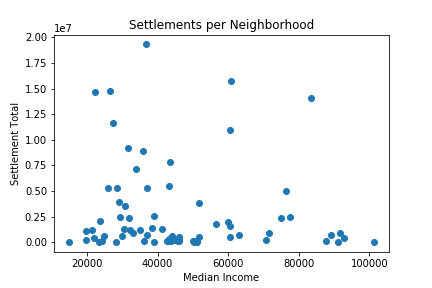
\includegraphics[width=0.5\textwidth]{settle1.png}
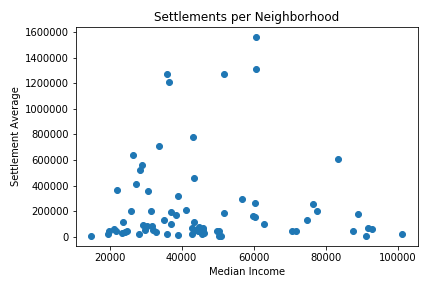
\includegraphics[width=0.5\textwidth]{settle2.png}
\end{figure}

\begin{table}[h!]
\centering
\caption{Table of Settlement Totals and Averages}
\label{table1}
\begin{tabular}{|l|l|l|l|}
\hline
name                   & median\_income & settlement\_total & settlement\_avg \\
\hline
Pullman                & \$36,622       & \$19,305,166      & \$1,206,572.88  \\
Garfield Ridge         & \$60,680       & \$15,752,302      & \$1,312,691.83  \\
Greater Grand Crossing & \$26,354       & \$14,717,153      & \$639,876.22    \\
North Lawndale         & \$22,132       & \$14,676,700      & \$366,917.50    \\
Near North Side        & \$83,382       & \$14,054,195      & \$611,051.96    \\
West Englewood         & \$27,203       & \$11,636,391      & \$415,585.39    \\
Morgan Park            & \$60,635       & \$10,939,698      & \$1,562,814.00  \\
Austin                 & \$31,478       & \$9,200,454       & \$200,009.87    \\
Brighton Park          & \$35,960       & \$8,890,000       & \$1,270,000.00  \\
Belmont Cragin         & \$43,425       & \$7,869,579       & \$462,916.41    \\
West Pullman           & \$33,758       & \$7,130,999       & \$713,099.90    \\
Archer Heights         & \$43,253       & \$5,464,057       & \$780,579.57    \\
Roseland               & \$37,084       & \$5,315,224       & \$196,860.15    \\
South Shore            & \$25,845       & \$5,285,493       & \$203,288.19    \\
South Chicago          & \$28,337       & \$5,240,992       & \$524,099.20    \\
Lake View              & \$76,424       & \$4,947,299       & \$260,384.16    \\
Douglas                & \$29,099       & \$3,947,750       & \$563,964.29    \\
Albany Park            & \$51,712       & \$3,820,198       & \$1,273,399.33  \\
South Lawndale         & \$30,603       & \$3,579,100       & \$357,910.00    \\
Hermosa                & \$39,057       & \$2,523,545       & \$315,443.13    \\
Auburn Gresham         & \$29,296       & \$2,486,123       & \$88,790.11     \\
Near South Side        & \$77,639       & \$2,416,971       & \$201,414.25    \\
Humboldt Park          & \$31,888       & \$2,378,756       & \$84,955.57     \\
West Town              & \$74,898       & \$2,360,001       & \$131,111.17    \\
West Garfield Park     & \$23,781       & \$2,095,389       & \$116,410.50    \\
\hline
\end{tabular}
\end{table}

\begin{table}[h!]
\centering
\caption{Table of Settlement Totals and Averages (cont)}
\label{table1}
\begin{tabular}{|l|l|l|l|}
\hline
name                   & median\_income & settlement\_total & settlement\_avg \\
\hline
Logan Square           & \$59,900       & \$1,966,484       & \$163,873.67    \\
Portage Park           & \$56,649       & \$1,772,718       & \$295,453.00    \\
Clearing               & \$60,483       & \$1,596,531       & \$266,088.50    \\
Gage Park              & \$38,444       & \$1,343,000       & \$167,875.00    \\
New City               & \$30,398       & \$1,279,741       & \$85,316.07     \\
Avalon Park            & \$41,221       & \$1,254,500       & \$209,083.33    \\
South Deering          & \$35,049       & \$1,198,949       & \$133,216.56    \\
East Garfield Park     & \$21,307       & \$1,189,522       & \$62,606.42     \\
Chatham                & \$32,074       & \$1,158,248       & \$55,154.67     \\
Englewood              & \$19,816       & \$1,091,807       & \$47,469.87     \\
Near West Side         & \$71,663       & \$917,044         & \$45,852.20     \\
Chicago Lawn           & \$32,944       & \$861,791         & \$35,907.96     \\
Loop                   & \$91,851       & \$857,830         & \$71,485.83     \\
Beverly                & \$89,038       & \$723,896         & \$180,974.00    \\
Rogers Park            & \$37,064       & \$723,000         & \$103,285.71    \\
Ashburn                & \$62,981       & \$718,560         & \$102,651.43    \\
Washington Heights     & \$43,990       & \$622,180         & \$51,848.33     \\
Woodlawn               & \$24,847       & \$592,000         & \$49,333.33     \\
Grand Boulevard        & \$29,811       & \$584,750         & \$53,159.09     \\
Irving Park            & \$51,713       & \$547,720         & \$182,573.33    \\
West Ridge             & \$46,008       & \$540,262         & \$67,532.75     \\
Jefferson Park         & \$60,384       & \$468,500         & \$156,166.67    \\
Washington Park        & \$21,869       & \$424,003         & \$42,400.30     \\
Lincoln Park           & \$92,870       & \$373,000         & \$62,166.67     \\
East Side              & \$43,305       & \$355,000         & \$118,333.33    \\
Avondale               & \$44,627       & \$243,503         & \$48,700.60     \\
Norwood Park           & \$70,706       & \$234,693         & \$46,938.60     \\
West Elsdon            & \$44,763       & \$222,000         & \$74,000.00     \\
O'Hare                 & \$46,065       & \$204,000         & \$51,000.00     \\
Fuller Park            & \$19,589       & \$200,000         & \$22,222.22     \\
McKinley Park          & \$43,736       & \$160,000         & \$53,333.33     \\
Lower West Side        & \$35,996       & \$150,694         & \$25,115.67     \\
Calumet Heights        & \$49,914       & \$142,500         & \$47,500.00     \\
Montclare              & \$42,769       & \$140,000         & \$70,000.00     \\
Edgewater              & \$46,103       & \$132,000         & \$33,000.00     \\
Uptown                 & \$45,661       & \$128,500         & \$21,416.67     \\
Armour Square          & \$24,140       & \$106,750         & \$35,583.33     \\
Mount Greenwood        & \$87,696       & \$93,000          & \$46,500.00     \\
West Lawn              & \$50,318       & \$92,500          & \$46,250.00     \\
Bridgeport             & \$42,951       & \$86,000          & \$21,500.00     \\
Burnside               & \$23,457       & \$30,000          & \$30,000.00     \\
Kenwood                & \$39,079       & \$23,000          & \$11,500.00     \\
Forest Glen            & \$101,237      & \$20,000          & \$20,000.00     \\
Oakland                & \$28,269       & \$18,500          & \$18,500.00     \\
Hegewisch              & \$50,252       & \$16,000          & \$8,000.00      \\
Riverdale              & \$14,916       & \$14,500          & \$7,250.00      \\
North Center           & \$91,197       & \$5,000           & \$5,000.00      \\
Hyde Park              & \$51,050       & \$5,000           & \$5,000.00     \\
\hline
\end{tabular}
\end{table}


\FloatBarrier
\pagebreak

\newpage


\section{Total and average cost of settlements by officer race}

To start, we looked at the races of the officers and got some statistics for the settlement cost for each officer by joining the settlement information with a table with the settlement id. Using Trifacta we grouped the information by race of the officer. We could then create columns for each of the races. The averages listed are only for settlements less than a million. This was to get a better understanding of what occurs in the typical case of a settlement without any large outliers.

\begin{figure}[h!]
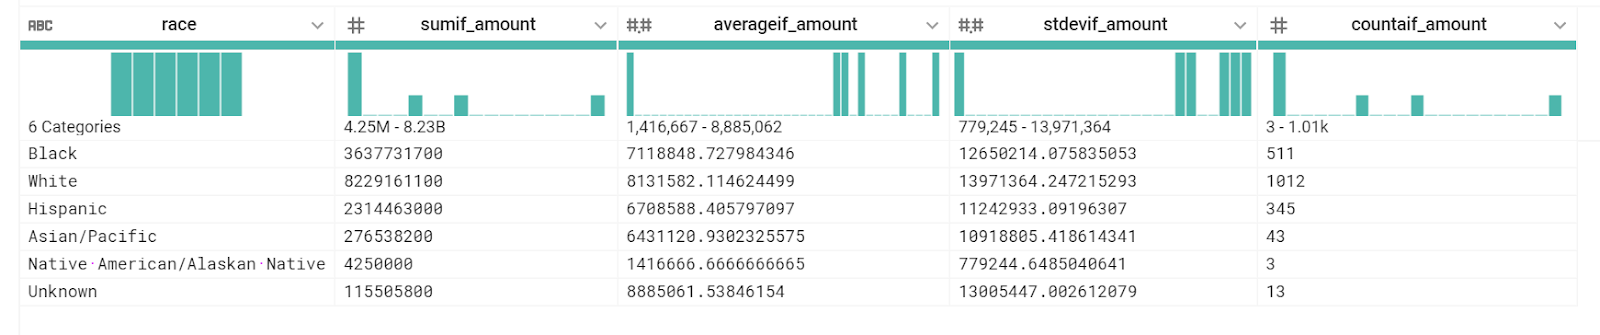
\includegraphics[width=\textwidth]{RaceTable.PNG}
\end{figure}

The table of average settlement values is below (table 3). The average white officer settlement costs the department around 81k which is 10k more than any other race. I would guess that when a white officer is involved, the police might pay out slightly larger settlements to somewhat avoid the bad press behind any race-related issues. As to why the Native American settlement value is so low, we're not really sure. There aren't many and so mostly we would assume it to be a fluke.


\begin{table}[h!]
\centering
\caption{Settlements by race}
\label{table3}
\begin{tabular}{|l|l|}
\hline
Officer Race	& Average Settlement\\
\hline
White                          & \$81,316  \\
Black                          & \$71,188  \\
Hispanic                       & \$67,085 \\
Asian/Pacific                  & \$64,311  \\
Native American/Alaskan Native & \$14,167  \\
Unknown                        & \$88,851 \\
\hline
\end{tabular}
\end{table}

\pagebreak

\section{Average age of officers involved in settlements}
Process: Join the data\_officer table to the officer table from the settlement database, then join with officer settlement to get the settlement ids, and finally join with the settlement table. From there, we calculate the age of each officer at the time of the settlement incident, then take the average.

Answer: 39.56 years old. For comparison, the average age of current officers in CPD is 44.5 years old, although I’d expect younger officers are more likely to be in the field and thus be involved in complaints/settlements. Just to break it down more, below is the average age by rank for current officers. As we'd expect, lower ranks skew younger, but actually don't quite fully explain the lower average age for officers involved in settlements, so it does seem that younger officers in general are more likely to be involved in an incident.

\begin{figure}[h!]
\centering
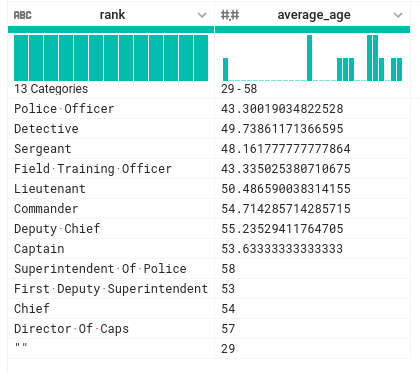
\includegraphics[scale=0.5]{ages.png}
\end{figure}


\section{Total allegations for each district vs total settlements}
Similar to the first question we used postgis to put the allegations and settlements into each neighborhood and counted them.

\begin{table}[h!]
\centering
\caption{Number of allegations and settlements per neighborhood}
\label{table4}
\begin{tabular}{|l|l|l|}
\hline
name                   & num\_allegations & num\_settlements \\
\hline
Austin                 & 7351             & 46               \\
Loop                   & 7260             & 12               \\
Near West Side         & 6025             & 20               \\
Near North Side        & 5723             & 23               \\
West Englewood         & 5245             & 28               \\
Auburn Gresham         & 4400             & 28               \\
North Lawndale         & 4111             & 40               \\
Humboldt Park          & 3971             & 28               \\
East Garfield Park     & 3773             & 19               \\
West Town              & 3739             & 18               \\
South Shore            & 3585             & 26               \\
Chicago Lawn           & 3437             & 24               \\
Englewood              & 3423             & 23               \\
Roseland               & 3259             & 27               \\
Douglas                & 3226             & 7                \\
Lake View              & 3166             & 19               \\
New City               & 3085             & 15               \\
Logan Square           & 3013             & 12               \\
Greater Grand Crossing & 2909             & 23               \\
Woodlawn               & 2751             & 12               \\
Rogers Park            & 2559             & 7                \\
Belmont Cragin         & 2559             & 17               \\
South Lawndale         & 2410             & 10               \\
Uptown                 & 2368             & 6                \\
Grand Boulevard        & 2352             & 11               \\
Near South Side        & 2325             & 12               \\
Chatham                & 2253             & 21               \\
South Chicago          & 2218             & 10               \\
West Garfield Park     & 2169             & 18               \\
Fuller Park            & 2105             & 9                \\
Pullman                & 2099             & 16               \\
West Pullman           & 1750             & 10               \\
Morgan Park            & 1633             & 7                \\
South Deering          & 1617             & 9                \\
Lower West Side        & 1568             & 6                \\
Lincoln Park           & 1548             & 6                \\
Bridgeport             & 1481             & 4                \\
North Center           & 1433             & 1                \\
Edgewater              & 1391             & 4                \\
Washington Heights     & 1353             & 12               \\
Garfield Ridge         & 1330             & 12               \\
Washington Park        & 1260             & 10               \\
Albany Park            & 1254             & 3                \\
Portage Park           & 1246             & 6                \\
\hline
\end{tabular}
\end{table}


\begin{table}[h!]
\centering
\caption{Number of allegations and settlements per neighborhood (cont)}
\label{table5}
\begin{tabular}{|l|l|l|}
\hline
name                   & num\_allegations & num\_settlements \\
\hline
Ashburn                & 1244             & 7                \\
West Ridge             & 1235             & 8                \\
Irving Park            & 1120             & 3                \\
Avondale               & 1020             & 5                \\
Hyde Park              & 989              & 1                \\
Archer Heights         & 983              & 7                \\
Brighton Park          & 965              & 7                \\
Gage Park              & 878              & 8                \\
Calumet Heights        & 827              & 3                \\
Jefferson Park         & 795              & 3                \\
O'Hare                 & 694              & 4                \\
Armour Square          & 678              & 3                \\
Kenwood                & 660              & 2                \\
West Lawn              & 659              & 2                \\
Avalon Park            & 657              & 6                \\
Beverly                & 640              & 4                \\
Norwood Park           & 627              & 5                \\
Clearing               & 593              & 6                \\
East Side              & 576              & 3                \\
McKinley Park          & 560              & 3                \\
Hermosa                & 553              & 8                \\
Mount Greenwood        & 482              & 2                \\
Riverdale              & 446              & 2                \\
Hegewisch              & 375              & 2                \\
West Elsdon            & 326              & 3                \\
Oakland                & 297              & 1                \\
Forest Glen            & 280              & 1                \\
Montclare              & 240              & 2                \\
Burnside               & 182              & 1               \\
\hline
\end{tabular}
\end{table}

For the most part, there seems to be a strong correlation between the two - as the number of allegations decreases, so does the number of settlements. There are quite a few inconsistencies however. Looking at the first few, the Loop stands out as having a lot of allegations and few settlements, while North Lawndale shows the opposite. The Loop is an interesting neighborhood in that it is extremely populated during the day with tourists and people going to work, but most do not actually live in the Loop. It might make sense that a person in the Loop would submit a complaint, but then maybe not stick around to follow through with court procedures. From the plot below, the Loop (bottom right) looks like it might be an outlier, but the rest of the neighborhoods do follow a roughly linear distribution.

\begin{figure}[h!]
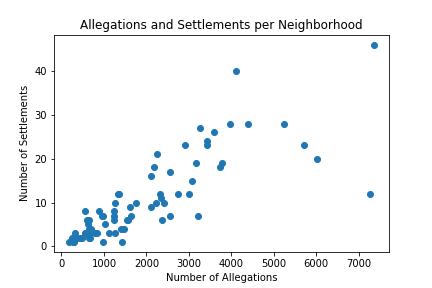
\includegraphics[width=\textwidth]{alleg_scatter.png}
\end{figure}



\end{document}